% Source for vignettes/model-overview-architecture-1.png.
% Only needs to be re-rendered when this file changes.
%
% Build the PDF with any LaTeX engine that supports TikZ, e.g.:
%   pdflatex model-overview-architecture.tex
%   tectonic model-overview-architecture.tex
%
% Convert to PNG with poppler:
%   pdftoppm -r 200 -png model-overview-architecture.pdf \
%            model-overview-architecture-1
%
% In R, `tinytex::install_tinytex()` provides a working LaTeX install.
\documentclass[tikz,border=12pt]{standalone}
\usepackage[T1]{fontenc}
\usepackage{lmodern}
\usetikzlibrary{
  arrows.meta,
  positioning,
  fit,
  backgrounds,
  shapes.geometric,
  calc
}

\definecolor{estblue}{HTML}{3B82F6}
\definecolor{estbluefill}{HTML}{DBEAFE}
\definecolor{optgreen}{HTML}{16A34A}
\definecolor{optgreenfill}{HTML}{DCFCE7}
\definecolor{fcastorange}{HTML}{EA580C}
\definecolor{fcastorangefill}{HTML}{FFEDD5}
\definecolor{wrapgrey}{HTML}{6B7280}
\definecolor{wrapgreyfill}{HTML}{F3F4F6}
\definecolor{datagold}{HTML}{CA8A04}
\definecolor{datagoldfill}{HTML}{FEF9C3}
\definecolor{internalbg}{HTML}{EFF6FF}
\definecolor{arrowcol}{HTML}{475569}

\begin{document}
\sffamily
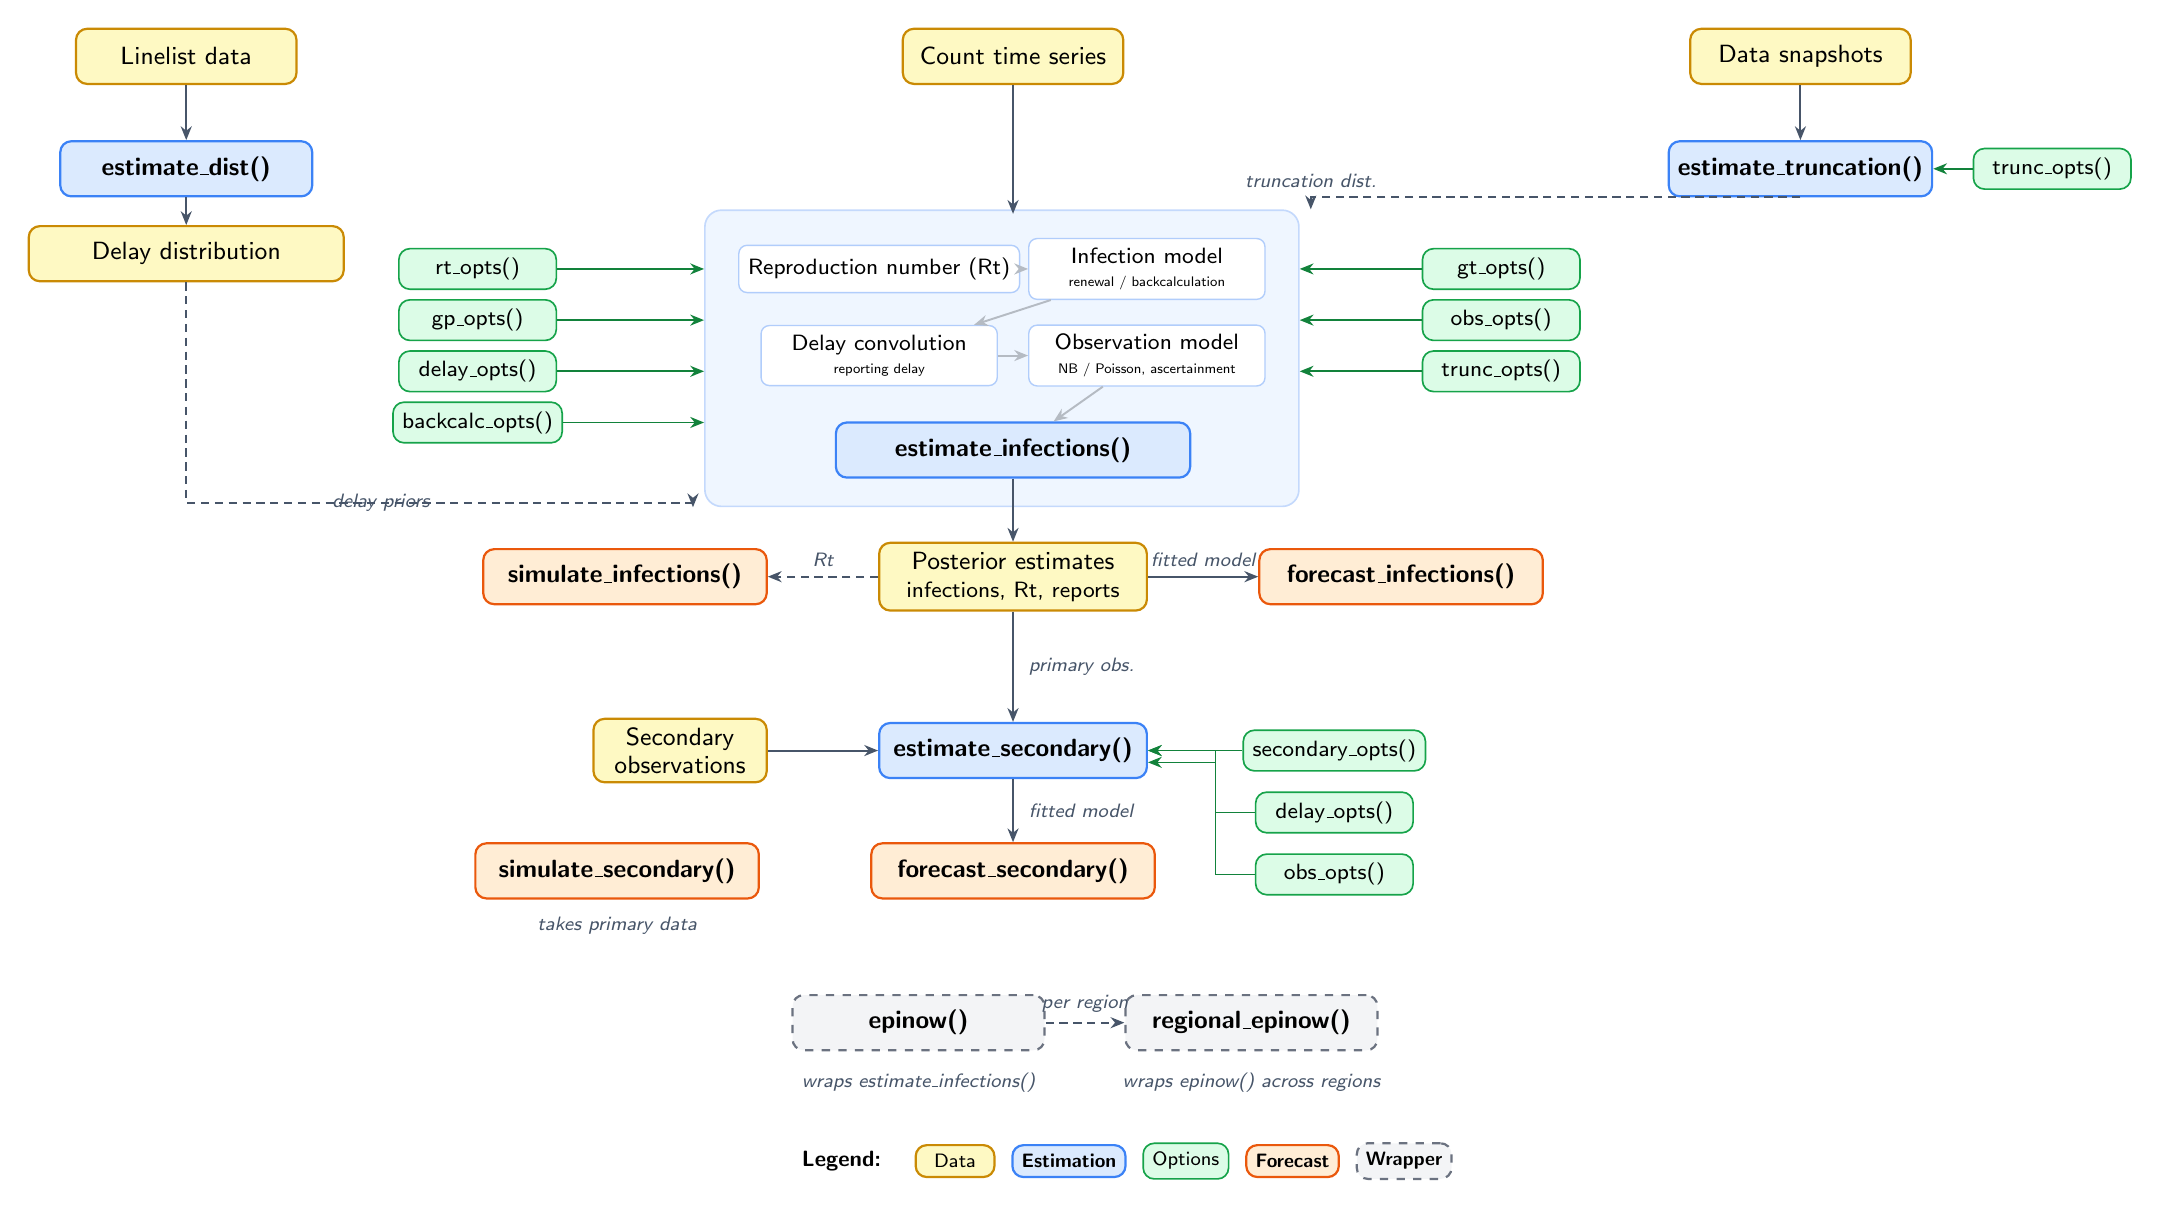
\begin{tikzpicture}[
  >={Stealth[length=5pt,width=4pt]},
  every node/.style={font=\sffamily\small},
  databox/.style={
    draw=datagold, fill=datagoldfill,
    rounded corners=4pt, minimum height=0.7cm,
    minimum width=2.8cm, align=center,
    line width=0.8pt
  },
  estbox/.style={
    draw=estblue, fill=estbluefill,
    rounded corners=4pt, minimum height=0.7cm,
    minimum width=3.2cm, align=center,
    line width=0.8pt, font=\sffamily\small\bfseries
  },
  optbox/.style={
    draw=optgreen, fill=optgreenfill,
    rounded corners=4pt, minimum height=0.5cm,
    minimum width=2.0cm, align=center,
    line width=0.6pt, font=\sffamily\footnotesize
  },
  fcastbox/.style={
    draw=fcastorange, fill=fcastorangefill,
    rounded corners=4pt, minimum height=0.7cm,
    minimum width=3.6cm, align=center,
    line width=0.8pt, font=\sffamily\small\bfseries
  },
  wrapbox/.style={
    draw=wrapgrey, fill=wrapgreyfill,
    rounded corners=4pt, minimum height=0.7cm,
    minimum width=3.2cm, align=center,
    line width=0.8pt, font=\sffamily\small\bfseries,
    dashed
  },
  intbox/.style={
    draw=estblue!40, fill=white,
    rounded corners=3pt, minimum height=0.6cm,
    minimum width=3.0cm, align=center,
    line width=0.5pt, font=\sffamily\footnotesize
  },
  arr/.style={
    ->, arrowcol, line width=0.7pt
  },
  darr/.style={
    ->, arrowcol, line width=0.7pt, densely dashed
  },
  optarr/.style={
    ->, optgreen!80!black, line width=0.6pt
  },
  lblstyle/.style={
    font=\sffamily\scriptsize\itshape, text=arrowcol
  }
]

% ==========================================
%  ROW 1: DATA INPUTS
% ==========================================
\node[databox] (cases) at (0, 0)
  {Count time series};
\node[databox] (snapshots) at (10, 0)
  {Data snapshots};
\node[databox] (linelist) at (-10.5, 0)
  {Linelist data};

% ==========================================
%  ROW 2: TRUNCATION (right column)
% ==========================================
\node[estbox, below=0.7cm of snapshots] (esttrunc)
  {estimate\_truncation()};
\node[optbox, right=0.5cm of esttrunc] (truncopt1)
  {trunc\_opts()};

\draw[arr] (snapshots) -- (esttrunc);
\draw[optarr] (truncopt1) -- (esttrunc);

% ==========================================
%  ESTIMATE_DIST (left column)
% ==========================================
\node[estbox, below=0.7cm of linelist]
  (estdist) {estimate\_dist()};

\draw[arr] (linelist) -- (estdist);

\node[databox, below=0.35cm of estdist,
  minimum width=4.0cm]
  (distout) {Delay distribution};

\draw[arr] (estdist) -- (distout);

% ==========================================
%  ESTIMATE_INFECTIONS BLOCK (centre)
% ==========================================
% Internal components — linear pipeline
\node[intbox] (rt) at (-1.7, -2.7)
  {Reproduction number (Rt)};
\node[intbox] (infmod) at (1.7, -2.7)
  {Infection model\\[-1pt]
    {\tiny renewal / backcalculation}};
\node[intbox] (delays) at (-1.7, -3.8)
  {Delay convolution\\[-1pt]
    {\tiny reporting delay}};
\node[intbox] (obsmod) at (1.7, -3.8)
  {Observation model\\[-1pt]
    {\tiny NB / Poisson, ascertainment}};

% Main function label at bottom of block
\node[estbox, minimum width=4.5cm] (estinf)
  at (0, -5.0) {estimate\_infections()};

% Background shading
\begin{scope}[on background layer]
  \node[
    fit=(rt)(infmod)(delays)(obsmod)(estinf),
    fill=internalbg, rounded corners=6pt,
    draw=estblue!30, line width=0.6pt,
    inner xsep=12pt, inner ysep=10pt
  ] (infbg) {};
\end{scope}

% Data arrow into block top
\draw[arr] (cases) -- (0, -2.0);

% Internal flow arrows (light)
% Rt → Infection model (renewal equation)
\draw[arr, arrowcol!40] (rt) -- (infmod);
% Infection model → Delay convolution
\draw[arr, arrowcol!40] (infmod) -- (delays);
% Delay convolution → Observation model
\draw[arr, arrowcol!40] (delays) -- (obsmod);
% Observation model → output
\draw[arr, arrowcol!40] (obsmod) -- (estinf);

% Delay priors: route down from distout, under
% the options, then right to the block bottom
\draw[darr] (distout.south)
  -- ++(0, -2.8)
  -| ([xshift=-4pt]infbg.south west)
  node[lblstyle, pos=0.25, left] {delay priors};

% Truncation distribution: clean L from esttrunc south
% across to the north-east corner of the infection block
\draw[darr] (esttrunc.south)
  -| ([xshift=4pt]infbg.north east)
  node[lblstyle, pos=0.5, above]
    {truncation dist.};

% ==========================================
%  OPTIONS — LEFT SIDE
% ==========================================
\node[optbox] at (-6.8, -2.7) (rtopts)  {rt\_opts()};
\node[optbox] at (-6.8, -3.35) (gpopts)  {gp\_opts()};
\node[optbox] at (-6.8, -4.0) (delayopts)
  {delay\_opts()};
\node[optbox] at (-6.8, -4.65) (backopts)
  {backcalc\_opts()};

% Arrows from left options to block boundary
\draw[optarr] (rtopts.east)
  -- (infbg.west |- rtopts);
\draw[optarr] (gpopts.east)
  -- (infbg.west |- gpopts);
\draw[optarr] (delayopts.east)
  -- (infbg.west |- delayopts);
\draw[optarr] (backopts.east)
  -- (infbg.west |- backopts);

% ==========================================
%  OPTIONS — RIGHT SIDE
% ==========================================
\node[optbox] at (6.2, -2.7) (gtopts)   {gt\_opts()};
\node[optbox] at (6.2, -3.35) (obsopts)  {obs\_opts()};
\node[optbox] at (6.2, -4.0) (truncopts)
  {trunc\_opts()};

% Arrows from right options to block boundary
\draw[optarr] (gtopts.west)
  -- (infbg.east |- gtopts);
\draw[optarr] (obsopts.west)
  -- (infbg.east |- obsopts);
\draw[optarr] (truncopts.west)
  -- (infbg.east |- truncopts);

% ==========================================
%  OUTPUTS
% ==========================================
\node[databox, below=0.8cm of estinf,
  minimum width=3.4cm] (posterior)
  {Posterior estimates\\[-1pt]
    {\footnotesize infections, Rt, reports}};

\draw[arr] (estinf) -- (posterior);

% ==========================================
%  FORECAST & SIMULATE INFECTIONS
% ==========================================
\node[fcastbox, right=1.4cm of posterior]
  (fcastinf) {forecast\_infections()};

\node[fcastbox, left=1.4cm of posterior]
  (siminf) {simulate\_infections()};

% forecast takes estimate_infections output
\draw[arr] (posterior) -- (fcastinf)
  node[lblstyle, midway, above] {fitted model};
% simulate can use estimated Rt for scenarios
\draw[darr] (posterior) -- (siminf)
  node[lblstyle, midway, above] {Rt};

% ==========================================
%  ESTIMATE_SECONDARY
% ==========================================
\node[estbox, below=1.4cm of posterior,
  minimum width=3.4cm]
  (estsec) {estimate\_secondary()};

\node[databox, left=1.4cm of estsec,
  minimum width=2.2cm]
  (secdata) {Secondary\\[-1pt]observations};

\draw[arr] (posterior) -- (estsec)
  node[lblstyle, midway, right, xshift=2pt]
    {primary obs.};
\draw[arr] (secdata) -- (estsec);

% Secondary options
\node[optbox, right=1.2cm of estsec]
  (secopts) {secondary\_opts()};
\node[optbox, below=0.25cm of secopts]
  (secdelay) {delay\_opts()};
\node[optbox, below=0.25cm of secdelay]
  (secobs) {obs\_opts()};

\draw[optarr] (secopts) -- (estsec);
\draw[optarr] (secdelay.west)
  -- ++(-0.5, 0) |- (estsec.east);
\draw[optarr] (secobs.west)
  -- ++(-0.5, 0)
  |- ([yshift=-0.15cm]estsec.east);

% ==========================================
%  FORECAST & SIMULATE SECONDARY
% ==========================================
\node[fcastbox, below=0.8cm of estsec]
  (fcastsec) {forecast\_secondary()};
\node[fcastbox, left=1.4cm of fcastsec]
  (simsec) {simulate\_secondary()};

% forecast takes estimate_secondary output
\draw[arr] (estsec) -- (fcastsec)
  node[lblstyle, midway, right, xshift=2pt]
    {fitted model};
% simulate is standalone (takes primary data)
\node[lblstyle, below=0.1cm of simsec]
  {takes primary data};

% ==========================================
%  WRAPPER LAYER
% ==========================================
\node[wrapbox, below=1.2cm of fcastsec,
  xshift=-1.2cm]
  (epinow) {epinow()};
\node[wrapbox, right=1.0cm of epinow]
  (regional) {regional\_epinow()};

\node[lblstyle, below=0.15cm of epinow]
  (epinowlbl)
  {wraps estimate\_infections()};
\node[lblstyle, below=0.15cm of regional]
  (reglbl)
  {wraps epinow() across regions};

\draw[darr] (epinow) -- (regional)
  node[lblstyle, midway, above] {per region};

% ==========================================
%  LEGEND
% ==========================================
\node[anchor=north west,
  font=\sffamily\footnotesize\bfseries] (legtitle)
  at ([yshift=-0.5cm]epinowlbl.south west)
  {Legend:};

\node[databox, minimum width=1.0cm,
  minimum height=0.35cm,
  font=\sffamily\scriptsize,
  right=0.3cm of legtitle.east, anchor=west]
  (leg1) {Data};
\node[estbox, minimum width=1.2cm,
  minimum height=0.35cm,
  font=\sffamily\scriptsize\bfseries,
  right=0.2cm of leg1] (leg2) {Estimation};
\node[optbox, minimum width=1.0cm,
  minimum height=0.35cm,
  font=\sffamily\scriptsize,
  right=0.2cm of leg2] (leg3) {Options};
\node[fcastbox, minimum width=1.0cm,
  minimum height=0.35cm,
  font=\sffamily\scriptsize\bfseries,
  right=0.2cm of leg3] (leg4) {Forecast};
\node[wrapbox, minimum width=1.0cm,
  minimum height=0.35cm,
  font=\sffamily\scriptsize\bfseries,
  right=0.2cm of leg4] (leg5) {Wrapper};

\end{tikzpicture}
\end{document}
